The DIRC detector is based on the concept of the Detection of Internally Reflected Cherenkov light (DIRC) produced in a solid radiator bar to identify charged particle. It is a special type of Cherenkov counter, which uses the unique properties of the Cherenkov radiation.

%ooOOooOOooOOooOOooOOooOOooOOooOOooOOooOOooOOooOOooOOooOOooOOooOOooOOooOOooOOoo%
%ooOOooOOooOOooOOooOOooOOooOOooOOooOOooOOooOOooOOooOOooOOooOOooOOooOOooOOooOOoo%
\section{Cherenkov Radiation}
Einstein postulated in his Theory of Relativity that the speed of light in a vacuum, $c$, is the limit of the velocity of massive particles. In an optically transparent medium, however, the speed at which light propagates is modified: $c_{med} = c/n$, where $n$ is the index of refraction of the medium. Pavel Cherenkov discovered in 1934 that massive particles moving through a medium faster than the speed of light in that medium emit light in the form of now-called Cherenkov radiation. Cherenkov was able to establish several interesting properties of this radiation: it is only emitted from charged particles above a certain velocity threshold $v > c/n$, the intensity is proportional to the particle's path length, emission is prompt, and the light is polarized with a continuous wavelength spectrum. Later in 1937 Ilya Frank and Igor Tamm theoretically formulated this radiation with fantastic agreement to Cherenkov's findings, and the three shared the 1958 Nobel Prize in Physics for their efforts \cite{CherenkovHistory}.

Further studies confirmed that Cherenkov radiation is emitted uniformly in azimuth ($\phi_c$) around the particle's direction of travel with the polar opening angle $\thetaC$ defined as
\begin{equation}
	\cos\thetaC = \frac{1}{\beta n(\lambda)},
	\label{eq:cherenkovformula}
\end{equation}
where $\beta = v_p/c$, $v_p$ is the particle's velocity, and the index of refraction is a function of the emitted photon wavelength. In a normal, dispersive optical medium the opening half-angle of the shock wave produced by the Cherenkov radiation, $\eta_C$ defined in Figure \ref{fig:cherenkovcone}, is not complementary to the Cherenkov angle. The relationship between the two is given by
\begin{equation}
	\cot\eta_C = \left[\frac{\diff}{\diff\omega}(\omega \tan\thetaC) \right]_{\omega_0} = \left[\tan\thetaC + \beta^2\omega n(\omega) \frac{\diff n}{\diff\omega}\cot\thetaC \right]_{\omega_0}
	\label{eq:openingangle}
\end{equation}
where $\omega_0$ is the central vale of the considered frequency range. Because the second term in (\ref{eq:openingangle}) is zero only for non-dispersive media the shock wave front is not perpendicular to the Cherenkov cone in real detectors.

\begin{figure}[ht]
	\centering
	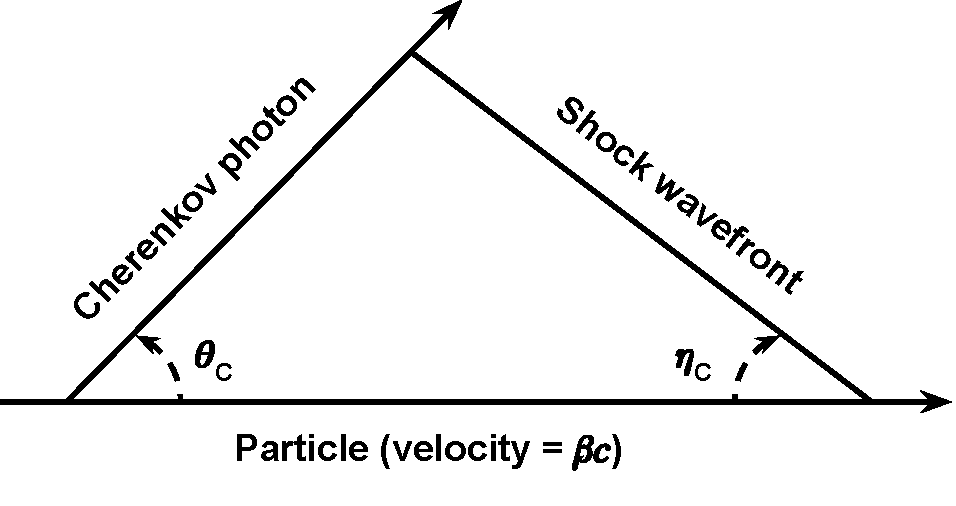
\includegraphics[scale=1]{figures/Cherenkov_cone.pdf}
	\caption{Illustration of the Cherenkov cone.}
	\label{fig:cherenkovcone}
\end{figure}

Because particles lose very little energy when radiating Cherenkov photons the emission is very weak. The number of photons $N_{photons}$ emitted per path length $L$ (in cm) by a moving particle with charge $z$ is given by the Frank-Tamm equation

\begin{equation}
	\frac{N_{photons}}{L} = \frac{\alpha^2 z^2}{r_e m_e c^2} \int \sin^2\thetaC (E) \diff E
	\label{eq:nphotons}
\end{equation}
where E is the photon energy in eV, the integral is taken over the region where $n(E)$ is greater than 1, and $\frac{\alpha^2 z^2}{r_e m_e c^2} = 370\unit{cm}^{-1}\unit{eV}^{-1}$.

%ooOOooOOooOOooOOooOOooOOooOOooOOooOOooOOooOOooOOooOOooOOooOOooOOooOOooOOooOOoo%
%ooOOooOOooOOooOOooOOooOOooOOooOOooOOooOOooOOooOOooOOooOOooOOooOOooOOooOOooOOoo%
\section{Applying the Cherenkov Effect to Particle ID}
In order to identify particle species one must know both the mass and charge of the particle in question. Because the Cherenkov angle encodes the particle's velocity it is, in principle, a simple matter to measure the particle's momentum with a tracking chamber as well as the velocity obtained from (\ref{eq:cherenkovformula}) to determine the mass and charge. Figure \ref{fig:angleseperation} shows how different particle species can be distinguished for a given momentum in fused silica.

Threshold Cherenkov counters are detectors used for particle identification (PID) by exploiting the fact that only particles above the threshold velocity $\beta > 1/n$ will emit Cherenkov photons. The information about a particle's velocity can be combined with momentum information from a tracking system to determine the mass as \cite{ParticleDetectionHandbook}

\begin{equation}
	m = \frac{p}{c} \sqrt{n^2 \cos^2\thetaC - 1}
	\label{eq:mass}
\end{equation}

\begin{figure}[ht]
	\centering
	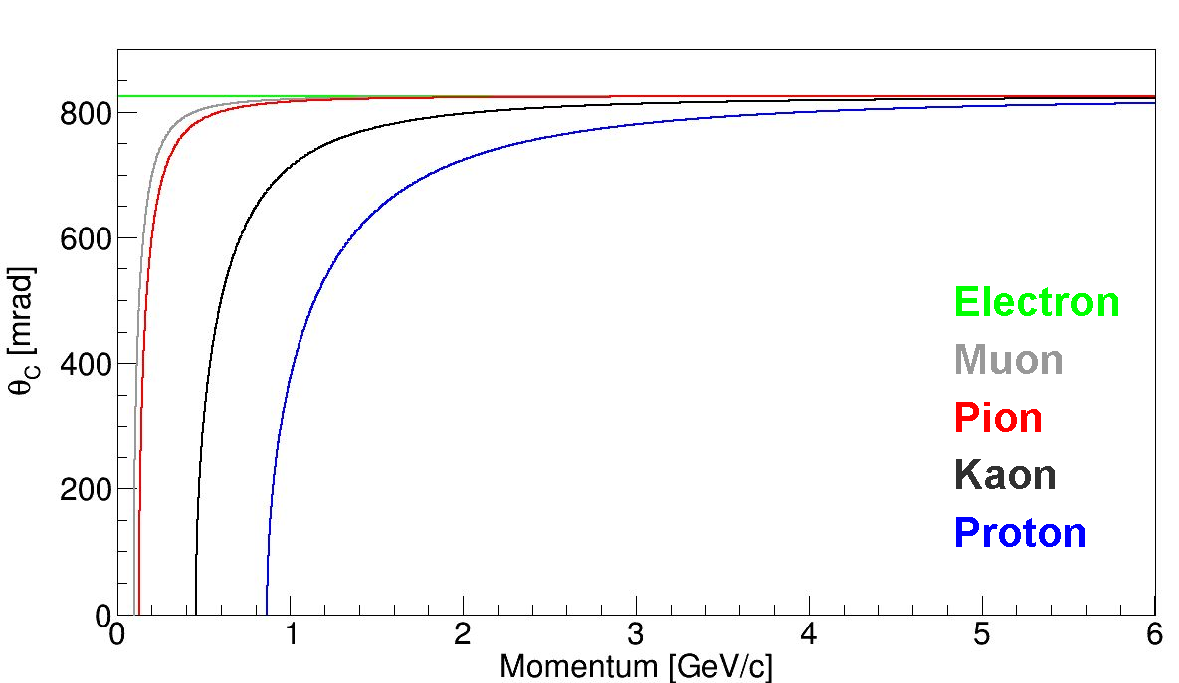
\includegraphics[scale=.8]{figures/angle_seperation_6.pdf}
	\caption{Particle momentum versus Cherenkov angle for different particle species in fused silica ($n \approx 1.473$).}
	\label{fig:angleseperation}
\end{figure}

%ooOOooOOooOOooOOooOOooOOooOOooOOooOOooOOooOOooOOooOOooOOooOOooOOooOOooOOooOOoo%
%ooOOooOOooOOooOOooOOooOOooOOooOOooOOooOOooOOooOOooOOooOOooOOooOOooOOooOOooOOoo%
\section{Ring Imaging Detectors}
Ring Imaging Cherenkov (RICH) detectors are desiged to efficiently identify and separate different particle species over a wide range of momenta. A basic RICH system is shown in Figure \ref{fig:richbasics}. 

\begin{figure}[ht]
	\centering
	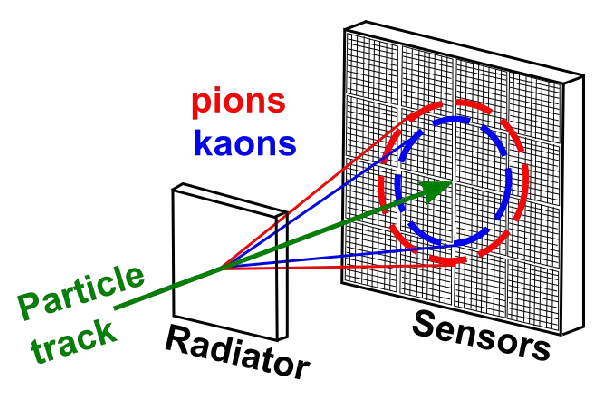
\includegraphics[scale=1]{figures/RICH.pdf}
	\caption{Schematic of a Proximity Focusing Ring Imaging Cherenkov (RICH) detector.}
	\label{fig:richbasics}
\end{figure}
A volume of radiator, either gaseous (e.g. $C_{4}F_{10}$) or solid (e.g. aerogel), is positioned upstream of an array of photosensors. A charged particle travelling through a thin radiator above the threshold velocity will continuously emit Cherenkov photons in a cone. The resulting image on the photosensor array is an annulus of thickness $L\tan\thetaC$, where $L$ is the distance the particle travelled inside the radiator, and  $\thetaC$ is the usual Cherenkov angle (Figure \ref{fig:richannulus}).
\begin{figure}[ht]
	\centering
	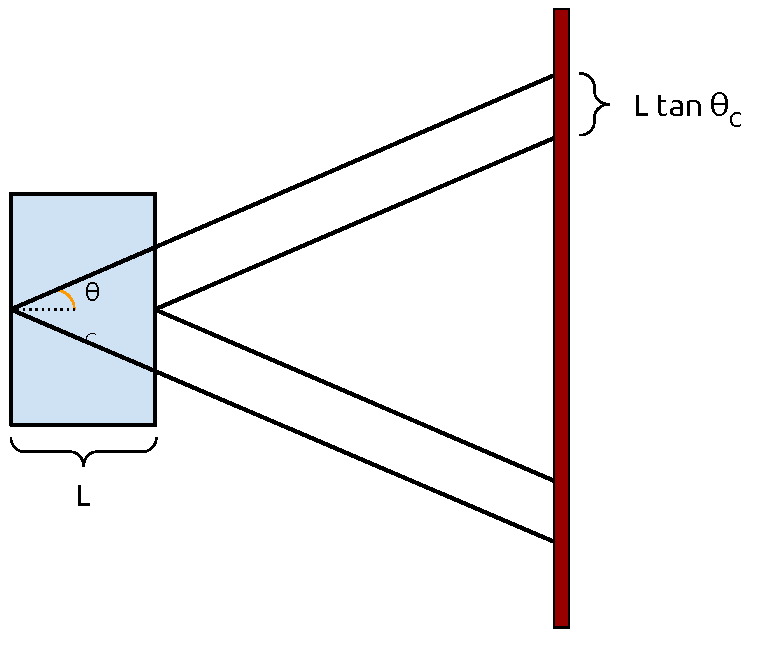
\includegraphics[scale=0.75]{figures/RICH_annulus.pdf}
	\caption{Annulus ring of RICH detector.}
	\label{fig:richannulus}
\end{figure}
PID can be done by measuring the average radius of the annulus and reconstructing the Cherenkov angle geometrically.


%ooOOooOOooOOooOOooOOooOOooOOooOOooOOooOOooOOooOOooOOooOOooOOooOOooOOooOOooOOoo%
%ooOOooOOooOOooOOooOOooOOooOOooOOooOOooOOooOOooOOooOOooOOooOOooOOooOOooOOooOOoo%
\section{DIRC Detectors}
The basic components of a DIRC detector are shown in Figure \ref{fig:dircbasics}.

\begin{figure}[ht]
	\centering
	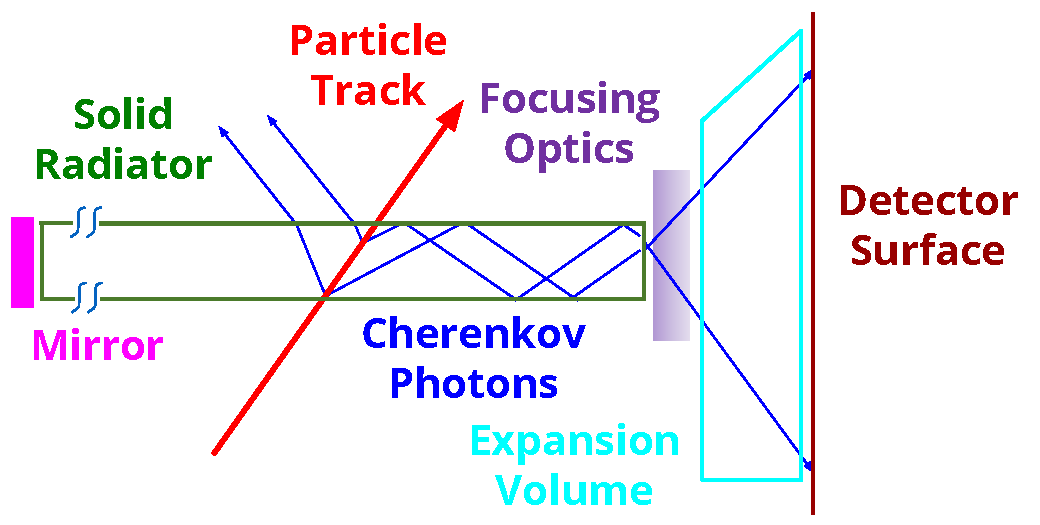
\includegraphics[scale=0.7]{figures/DIRC_components.pdf}
	\caption{The basic components of a DIRC detector: a solid radiator, typically fused silica (green); a mirror to redirect backward-going photons (pink); optional focusing optics (purple); an expansion volume to allow photons to separate in space (cyan); and a detector surface to record the position and arrival time of Cherenkov photons (maroon).}
	\label{fig:dircbasics}
\end{figure}

\subsection{DIRCs in Future Experiments}
EIC, PANDA, Bell, ToRCH, GlueX
